
\documentclass[a4paper,12pt]{article}

\usepackage[T1]{fontenc}
\usepackage{times}
\usepackage[swedish,english]{babel}
\usepackage[utf8]{inputenc}
\usepackage{dtklogos}
\usepackage{wallpaper}
\usepackage[absolute]{textpos}
\usepackage[top=2cm, bottom=2.5cm, left=3cm, right=3cm]{geometry}
\usepackage{appendix}
\usepackage[nottoc]{tocbibind}

\setcounter{secnumdepth}{3}
\setcounter{tocdepth}{3}

\usepackage{sectsty}
\sectionfont{\fontsize{14}{15}\selectfont}
\subsectionfont{\fontsize{12}{15}\selectfont}
\subsubsectionfont{\fontsize{12}{15}\selectfont}

\usepackage{csquotes} % Used to handle citations

\renewcommand{\thetable}{\arabic{section}.\arabic{table}}  
\renewcommand{\thefigure}{\arabic{section}.\arabic{figure}}

\usepackage{array}
\newcolumntype{L}[1]{>{\raggedright\let\newline\\\arraybackslash\hspace{0pt}}m{#1}}
 

%----------------------------------------------------------------------------------------
%	
%----------------------------------------------------------------------------------------
\newsavebox{\mybox}
\newlength{\mydepth}
\newlength{\myheight}

\newenvironment{sidebar}%
{\begin{lrbox}{\mybox}\begin{minipage}{\textwidth}}%
{\end{minipage}\end{lrbox}%
 \settodepth{\mydepth}{\usebox{\mybox}}%
 \settoheight{\myheight}{\usebox{\mybox}}%
 \addtolength{\myheight}{\mydepth}%
 \noindent\makebox[0pt]{\hspace{-20pt}\rule[-\mydepth]{1pt}{\myheight}}%
 \usebox{\mybox}}

%----------------------------------------------------------------------------------------
%	Title section
%----------------------------------------------------------------------------------------
\newcommand\BackgroundPic{
    \put(-2,-3){
    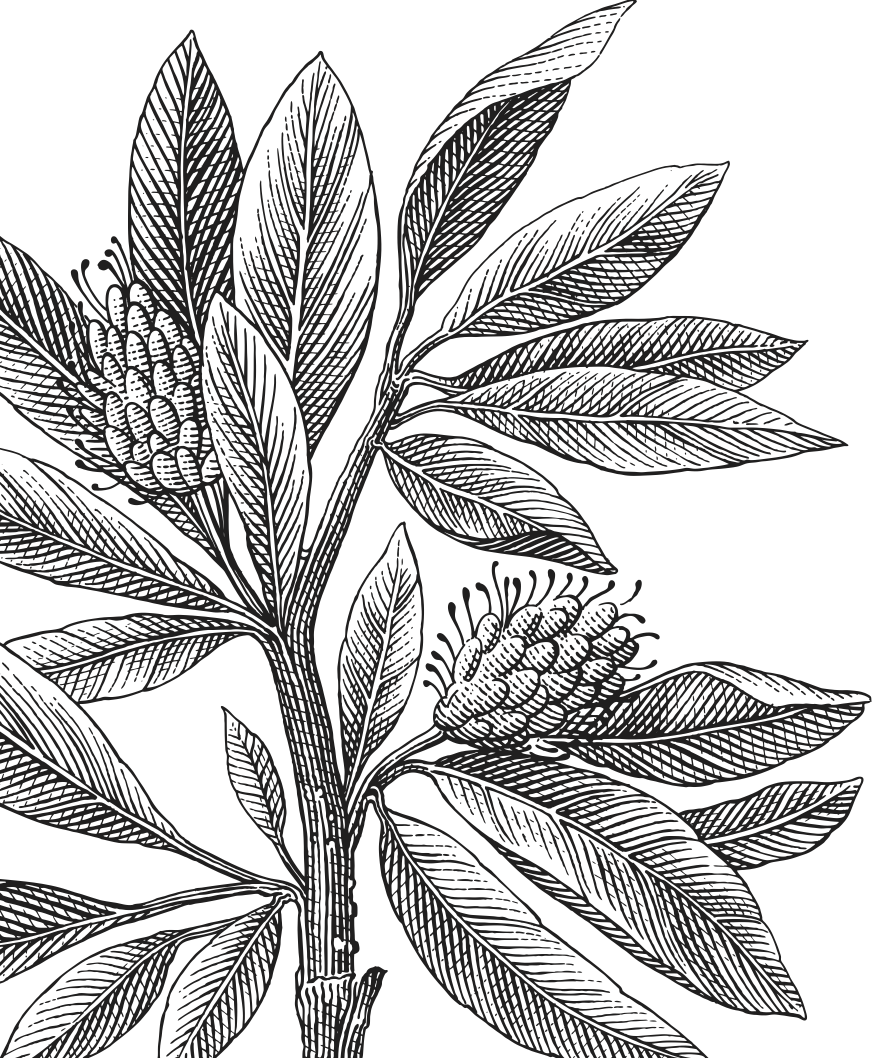
\includegraphics[keepaspectratio,scale=0.3]{img/lnu_etch.png} % Background picture
    }
}
\newcommand\BackgroundPicLogo{
    \put(30,740){
    
\includegraphics[keepaspectratio,scale=0.10]{img/logo.png} % Logo in upper left corner
    }
}

\title{	
\vspace{-8cm}
\begin{sidebar}
    \vspace{10cm}
    \normalfont \normalsize
    \Huge Report \\
    \vspace{-1.3cm}
\end{sidebar}
\vspace{3cm}
\begin{flushleft}
    \huge Project Course in Computer Science\\ 
    \it \LARGE - Test Case document
\end{flushleft}
\null
\vfill
\begin{textblock}{6}(10,13)
\begin{flushright}
\begin{minipage}{\textwidth}
\begin{flushleft} \large
\emph{Author:} Quasim Aljbarah, Michael Johansson, Tadas Lisauskas, Zeyuan Li, Robin Reijo and Robin Stempa\\ 
\emph{Supervistor:} Ola Petersson\\ 
%\emph{Examiner:} Dr.~Mark \textsc{Brown}\\ % Examiner (course manager)
\emph{Semester:} VT 2016\\ % 
\emph{Subject:} 1DV508\\ % Subject area
\end{flushleft}
\end{minipage}
\end{flushright}
\end{textblock}
}

\date{} 

\begin{document}
\pagenumbering{gobble}
\newgeometry{left=5cm}
\AddToShipoutPicture*{\BackgroundPic}
\AddToShipoutPicture*{\BackgroundPicLogo}
\maketitle
\restoregeometry
\clearpage
%----------------------------------------------------------------------------------------
%	Abstract
%----------------------------------------------------------------------------------------
\selectlanguage{swedish}


\newpage





\newpage
\pagenumbering{gobble}
\tableofcontents 
\newpage
\pagenumbering{arabic}
\section{Revision History}

\begin{table}[htbp]
	\centering
	\begin{tabular}{|L{3cm}|L{6cm}|L{4cm}|}
		\hline
		\textbf{Change} & \textbf{Description} & \textbf{Name and Date} \\ \hline
	Created the test case document  & Created the document and wrote down all the tests & Robin Reijo 22/4 - 2016\\ \hline
		Created Revision history table	&       included a revision history table to the document           &     Michael Johansson, 22/4 - 2016               \\ \hline
		Updated document 	& updated the document with the stuff we got on the seminar              &   Michael Johansson 8/5 - 2016                   \\ \hline
		&		&	  \\ \hline
	\end{tabular}
\end{table}
\newpage


\section{Introduction}
The purpose of this test case document is to showcase what they system shall be tested upon. For this purpose we use tables organize the work. Where you can look up what tests there is and requirements we put up for the intended test, and also how to test it and what we should come to expect of each of the tests.

\section{Test Cases - general}
\begin{tabular}{ |p{0.8cm}|p{0.8cm}|p{3.8cm}|p{3.8cm}|p{3.8cm}|  }
	\hline
	\multicolumn{5}{|c|}{Test Cases} \\
	\hline
	Test& ID & Requirements &How to test&Expected result\\
	\hline
	1 & 1. & The webshop must contain any number of products    & Search for an empty string in the search bar to get all products in the database & Should show products on the result page.\\
	\hline
	2  & 1.1 &All information regarding the product is stored in the database.   & Log in as admin and go to add new product, add information in the field and press add button & The added product should be shown in the database.\\
	\hline
	3 & 1.2 &A product shall contain product name, category, quantity, price, description and an image.    &Search for an empty string in the search bar to get all products in the database and check so no fields are missing & The product should contain all of the requirements.\\
	\hline
	4 & 1.3 & A placed order will be placed in the database  & Add products to your cart, from there click the checkout button and from that page click purchase  & Order should be able to be checked with the Ordernumber from Orderstatus page \\
	\hline
	5 & 1.3.1& Quantity changes made will be updated in database& Do as in test 4 to place an order with one quantity of the product & Quantity should updated with minus 1 in the database\\
	\hline

	
	
	
\end{tabular}
	\newpage
	\section{Test Cases - Customer}
\begin{tabular}{ |p{0.8cm}|p{0.8cm}|p{3.8cm}|p{3.8cm}|p{3.8cm}|  }
	\hline
	\multicolumn{5}{|c|}{Test Cases} \\
	\hline
	Test& ID &Requirements &How to test&Expected result\\
	\hline

	6    & 2. &A customer shall be able to browse product  & Search for a product and then click the product to come to its page & Should come to the specific products page\\
	\hline
	7    & 2. &A customer shall be able to browse product  & Go into a category and press a product & Should come to the specific products page\\ \hline
		8    & 2. &A customer shall be able to browse product  & Press a product in the new section of the frontpage  & Should come to the specific products page\\
	\hline
	9 &2.1.1& A customer shall be able to show products by category  & Click a category to show category specific products   & Should show product by category \\
	\hline
	10 & 2.2 &A customer shall be able to put a product in the shopping cart & Search for a product, add it to the cart and press go to cart & Should show newly added product. \\
	\hline
	 11 &2.2.1& A customer shall be able to change quantity while in the shoping cart. & Add a product to the cart then change quantity on the product by pressing on the quantity button and change to desired number. & Should update products in cart and change the quantity of the product \\
	\hline
	12 &	2.2.2 &A customer shall be able to remove a product with one click& Press the remove button at the desired product. & Product should be removed from the shopping cart. \\
	\hline
	 13 &2.3 &A customer shall be able to make an order & Go to shoping cart page, fill in the form with personal information and press purchase. & Customer should be able to see the placed order when going to customers individual page with its ordernumber.\\
	\hline
	 14 &2.3.1 & A customer shall be given an auto generated order number & Press purchase on the order form. & Should give the customer the number. \\
	
	\hline
	 15 &2.3.2 &A customer shall be able to view the status on his or her order. & Use the auto generated number to get to the page. & Should show the status of the order. \\
	\hline
	
\end{tabular}


	\newpage
	\section{Test Cases - Administrator}
	
		\begin{tabular}{ |p{0.8cm}|p{0.8cm}|p{3.8cm}|p{3.8cm}|p{3.8cm}|  }
			\hline
			\multicolumn{5}{|c|}{Test Cases} \\
			\hline
			Test& ID & Requirements &How to test&Expected result\\
			\hline
			
			 16 & 3.2.2 &Admin shall be able to change information about a product & Log in to admin page and press edit product, change a field and press edit & Should show newly added information of the product when it is viewed. \\
			\hline
			 17 &3.2.3 & Admin shall be able to add a category & Log in to admin page and press add category, then add a category & New category should be visible when adding a new product or at the category list \\
			\hline
			18 & 3.2.3 &Admin shall be able to remove a category & Log in to admin page and press edit category, remove a category & Removed category must be removed from category list \\
			\hline
			19 &3.2.3 &Admin shall be able to edit a category & Log in to admin page and press edit category, change a category & New category information should be visible when adding a new product or at the category list \\
			\hline
			 20 & 3.3 &Admin shall be able to add new admin accounts & Add a new admin account on the add new admin page & The new admin account should be visible in the database and an admin should be able to login using the new details.\\
			\hline
			 21& 3.4 &Admin shall be able to remove an admin account & remove a admin account on the edit admin page & The admin account should not be visible in the database and admin cant login. \\
			\hline
			 22& 3.4 &Admin shall be able to edit an admin accounts password & edit a admin account password on the edit admin page & The admin should only be able to log in with the new password \\
			 \hline
			 23 &3.5 &Admin shall be able to view all order of all customers. & Login into admin system, all order appear on admin edit orders page. & Should display all the orders made by customers \\
			\hline
			
			24 & 3.5.1 & Admin shall be able to update status on every order & Login as admin, go to the targeted customers random generated number ordered page and change status to new shipped, delayed and delivered and returned & Should show newly updated status on show all order page and individual order page. \\ 
			\hline
			
			
		\end{tabular}
		
			
		

	

\end{document}
